\chapter{Implementacja}
\label{implementacja}

\section{Specyfikacja wymagań}
\label{specyfikacja-wymagan}

\subsection{Wymagania funkcjonalne}
Użytkownikiem aplikacji jest administrator lub osoba posiadająca dużą kolekcję plików.
Wymagane funkcjonalności:
\begin{itemize}
\item Możliwość wyboru katalogu zawierających pliki wymagające zmiany nazw
\item Udostępnienie filtrów glob pozwalających na automatyczną selekcję plików
%\item Sortowanie wybranych plików za pomocą metawyrażeń
\item Możliwość ekstrakcji metadanych z~plików audio (MP3)
%  \begin{itemize}
%  \item MP3
%  \item PNG
%  %\item 
%  \end{itemize}
\item Wybór operacji na samych plikach lub pełnych ścieżkach (wraz z~katalogami)
\item Automatyczna iteracja względem wybranych plików i~zmiana ich nazwy
%\item Notyfikacja o~powtarzających się identyfikatorach plików
%\item Notyfikacja o~możliwych problemach z~kompatybilnością spowodowanych zastosowanym zestawem znaków
\item Notyfikacja o~błędach ekstrakcji metadanych
%\item Zachowywanie konfiguracji programu między uruchomieniami
\end{itemize}

\subsection{Wymagania niefunkcjonalne}
\begin{itemize}
\item Minimalistyczny, skalowalny interfejs użytkownika
\item Aplikacja powinna być przenośna na poziomie kodu źródłowego między platformami zgodnymi ze standardem \texttt{POSIX}.
%z rodziny Microsoft Windows jak i~
\end{itemize}

%\section{Projekt}
%\label{projekt}

\section{Wykorzystane biblioteki}
\label{wykorzystane-biblioteki}

\subsection{SigC++}
\begin{wrapfigure}{r}{0.4\textwidth}
\begin{center}

\includegraphics[scale=0.50]{img/sigcpp_logo.png}
\end{center}
\caption{Logo biblioteki SigC++}
\end{wrapfigure}
\par
SigC++ jest biblioteką dla języka C++ implementującą bezpieczny (ze względu na typy) mechanizm sygnałów.
Sygnały (zdarzenia) są wysokopoziomowym odpowiednikiem wywołań zwrotnych używanych do wstrzykiwania kodu programisty-użytkownika do istniejącej implementacji. W~językach niskopoziomowych, takich jak C często stosuje się do tego celu wskaźniki do funkcji, jednak ich niskopoziomowa natura może powodować trudne do wykrycia błędy spowodowane przekazaniem złego typu wskaźnika lub błędnej jego sygnatury. Biblioteka udostępnia wysokopoziomowe szablony obiektów sygnałów jak i~interfejsy do zastosowania w~klasach użytkownika, ułatwiające w~znaczny sposób zarządzanie podpiętymi zdarzeniami.\\
\par
SigC++ jest często używana w~projektach GUI takich jak pulpit GNOME; w~takim też celu zostanie ona użyta w~aplikacji MRU.

\subsection{\texttt{boost::filesystem}}
\par
Biblioteka \texttt{boost::filesystem} pozwala na niezależny od systemu operacyjnego dostęp do drzewa katalogów\cite{wiecej-niz-cpp-boost}. Ze względu na swoją uniwersalność została użyta w modułach BoostInput oraz BoostOutput, które są domyślnymi sterownikami wejścia/wyjścia w~aplikacji MRU.

%\subsection{\texttt{boost::property\_tree}}
%\par
%\texttt{boost::property\_tree} jest drzewiastym (hierarchicznym) kontenerem ogólnego przeznaczenia\footnote{Z założenia biblioteka \texttt{boost::property\_tree} została stworzona do reprezentacji struktury ogólnych plików konfiguracyjnych lecz nic nie stoi na przeszkodzie aby traktować ją jako ogólny kontener}, który posłuży jako główne źródło informacji o~wtyczkach i~samym rdzeniu aplikacji MRU.

%\subsection{\texttt{boost::program\_options}}
%\par
%Biblioteka \texttt{boost::program\_options} udostępnia wygodny i~rozszerzalny parser argumentów przekazanych programowi z~linii komend.

\subsection{wxWidgets}
\begin{wrapfigure}{r}{0.4\textwidth}
\begin{center}

\includegraphics[scale=0.50]{img/wxwidgets_logo.png}
\end{center}
\caption{Logo biblioteki wxWidgets}
\end{wrapfigure}

\par
wxWidgets jest wieloplatformową biblioteką do tworzenia graficznych interfejsów użytkownika (ang. GUI). W~projekcie została wykorzystana do stworzenia wtyczki interfejsu (ui module) wxWidgetsUi. wxWidgets udostępnia i~pozwala tworzyć przenośny zestaw klas kontrolek, które są tłumaczone na natywne kontrolki środowiska uruchamiającego aplikacje.

\subsection{ICU}
\par
ICU --- International Components for Unicode" --- jest biblioteką opracowaną przez IBM wspierającą lokalizacje, globalizacje i~umożliwiającą operacje na łańcuchach znaków w~kodowaniach UTF.\\
Jako że główne operacje w~aplikacji MRU przeprowadzane są na łańcuchach znaków, istotne jest aby wykonywane były one z~należytą precyzją. ICU jest najbardziej zaawansowaną, ogólnie dostępną biblioteką tego typu z~długą historią zastosowań.

\subsection{CppUnit}
\par
Aby zapewnić najwyższą jakość produkowanego kodu i zmniejszyć ryzyko błędów (w tym opartych na regresji), większość z modułów i interfejsów aplikacji została zaprojektowana i zaimplementowana z użyciem testów jednostkowych. Testy zostały napisane w oparciu o bibliotekę \texttt{CppUnit}, która ułatwia ich uruchamianie, debugowanie i zarządzanie nimi.

\subsection{TagLib}
TagLib jest biblioteką pozwalającą na ekstrakcje metadanych z~wielu typów plików multimedialnych. W MRU została użyta w implementacji metatagu Audio umożliwiającego dostęp do informacji o~tytule, roku wydania, a~także wykonawcy i~albumie do którego należy utwór muzyczny.

\section{Rdzeń aplikacji - klasa MruCore}
Rdzeniem aplikacji jest klasa \texttt{MruCore} stanowi ona interfejs do całej funkcjonalności programu i~udostępnia informacje o~jego działaniu.
\par
Klasa \texttt{MruCore} zawiera metody umożliwiające wtyczkom UI na kontrolę pracy programu bez implementacji powtarzalnej logiki, a~sygnały zdefiniowane w~klasie dostarczają informacji zwrotnej o~pracy aplikacji.

\section{glue\_cast - łącznik technologii}
Jako że w~aplikacji zostały wykorzystane różne biblioteki, wprowadziły one wiele wymagań co do obsługiwanych typów danych.
Biblioteka ICU korzysta głównie z~klas takich jak \texttt{UnicodeString} podczas gdy biblioteki \texttt{boost} zostały oparte na strukturach ze standardowej biblioteki \texttt{STL} takich jak \texttt{std::string}. Do tego dochodzi niskopoziomowa warstwa API systemu operacyjnego która często operuje na surowych łańcuchach znaków --- \texttt{const char *}.
\par
Aby ułatwić konwersję między różnymi redundantnymi typami danych, został opracowany szablon \texttt{glue\_cast} podobny w~zastosowaniu do wbudowanych w~język język rzutowań takich jak \texttt{dynamic\_cast} czy \texttt{reinterpret\_cast}.

\begin{lstlisting}[caption={ glue.hpp}, language=C++]
template<typename DstType, typename SrcType> inline
DstType
glue_cast(const SrcType &a_value)
{
  return DstType(a_value);
}
\end{lstlisting}

\par
Przedstawiona powyżej generyczna implementacja szablonu często jest niewystarczająca lecz dzięki odpowiednim specjalizacjom, w całym programie można wykorzystywać jednorodną składnie odpowiadającą za rzutowania.
\clearpage
\begin{lstlisting}[caption={ Fragment glue\_impl.hpp --- specjalizacja dla std::wstring i~wxString}, language=C++]
template<> inline
wxString
glue_cast<wxString, std::wstring>(const std::wstring &a_value)
{
  return wxString(a_value.c_str(), wxConvUTF8);
}

template<> inline
std::wstring
glue_cast<std::wstring, wxString>(const wxString &a_value)
{
  return std::wstring(a_value.wc_str());
}

\end{lstlisting}

\par
Dzięki wykorzystaniu szablonów nie ma potrzeby tworzenia nowych funkcji konwersji, a~całość wygląda bardziej spójnie, a także jest łatwiejsza w~utrzymaniu (powtarzający się kod został zamknięty w specjalizacjach). Dodatkowym atutem użytego rozwiązania jest jego uniwersalność --- wybrane specjalizacje można wykorzystać w~jakimkolwiek projekcie używających specjalizowanych typów. Dodawanie nowych konwersji sprowadza się do dopisania kolejnej pary szablonów.

\section{Wyrażenia zawierające metatagi}
Najważniejszym elementem projektu MRU są metatagi wraz metawyrażeniami na które się składają.
Metawyrażenia używane są jak wzorzec (szablon) na podstawie którego generowane są kolejne nazwy plików.

\par
Za każdym razem gdy MRU zmienia plik na którym operuje, metawyrażenie jest ewaluowane. Każde wystąpienie tagu jest przekładane na wywołanie odpowiedniej metody na obiekcie wtyczki, a~rezultat tego wywołania jest wstawiany w~miejsce wystąpienia tagu.
Metatagi są reprezentacjami wywołań do odpowiadającym im wtyczek.

\begin{wrapfigure}{r}{0.4\textwidth}
\begin{center}

\includegraphics[scale=0.50]{img/metatag_sample.png}
\end{center}
\caption{Metatag z~wyróżnionymi elemetami na niego się składającymi}
\end{wrapfigure}

\par
Metatag jest identyfikatorem wprowadzonym do zwykłego tekstu, składającym się z~czterech elementów które nie mogą zostać rozdzielone białymi znakami. Metatag rozpoczyna się od symbolu procent --- '\%' --- po którym następuje nazwa metatagu składająca się ze znaków alfanumerycznych alfabetu łacińskiego\footnote{Z technicznego punktu widzenia nic nie stoi na przeszkodzie aby do zapisu nazwy metataga zastosować pełen zestaw znaków, lecz ze względu na globalizacje nie wszyscy użytkownicy potrafili by używać każdej nazwy.}.
Po nazwie następuje para nawiasów --- '(' wraz z~')' --- zawierających opcjonalnie listę parametrów inicjalizacyjnych metatag. Nie istnieją ograniczenia co do zawartości listy inizjalizującej --- może ona zawierać pełen zakres znaków.
%włączając to znaki zakończenia listy (nawiasy zamykające) o~ile są odpowiednio oznaczone\footnote{Aby zignorować interpretację znaku specjalnego w~metawyrażeniu, można użyć ogólnie znanego schematu wyłączania znaków --- poprzedzania ich symbolem '\textbackslash'}.
Ostatnim elementem jest opcjonalny zakres działania metatagu --- jest to obszar zawierający się między parą nawiasów klamrowych ('\{' oraz '\}') który sam w~sobie jest metawyrażeniem. Dzięki temu, efekty metatagów mogą się na siebie nakładać.

\begin{figure}[h]
\begin{center}
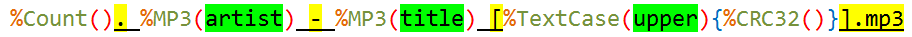
\includegraphics[scale=0.55]{img/metatag_expr2.png}
\end{center}
\caption{Przykładowe metawyrażenie wraz z~wyróżnionymi elementami metatagów}
\label{metatag-expr}
\end{figure}

\par
Parsowanie metawyrażenia rozpoczyna się od tokenizacji. Tekst wejściowy rozdzielany na grupy które mogą składać się z pojedynczych symboli (użytych w metatagu) bądź łańcucha znaków niezawierającego w/w symboli.

\par
Następnym krokiem jest przekazanie listy powstałej przy tokenizacji do leksera, który przypisuje umowne symbole dla konkretnych jej elementów tworząc tym samym listę tokenów. Na tym etapie każdy token zawiera tekst (bądź pojedynczy symbol) z którego powstał, typ i pozycję w oryginalnym tekście wejściowym.

\par
Ostatnim etapem jest interpretacja listy tokenów przez parser generujący obiekty metawyrażeń (gotowe do wykonania po zapewnieniu implementacji wtyczek metatagów).
Jako parsowanie ogólnie nie należy do łatwych zadań (nawet w przypadku tak niewielkiej liczby tokenów), do interpretacji poprawności kolejności tokenów została użyta specjalna maszyna stanów.
Programista deklaruje jedynie poprawne i końcowe stany które maszyna może przyjąć, możliwe przejścia między stanami oraz funkcje które powinny być wywołane przy wejściu/opuszczeniu stanu.
Po przekazaniu listy tokenów do maszyny stanów, wywołuje ona odpowiednie metody (sprecyzowane wcześniej przez programistę) które budują drzewo wywołań możliwe do zamknięcia w obiekt metawyrażenia.
W przypadku błędu (nie poprawnej sekwencji tokenów bądź zakończeniu listy w stanie niekońcowym) maszyna wyrzuca wyjątek z tokenem który powoduje problem.

\par
Klasy tokenizera, leksera, parsera oraz maszyny stanów zostały zaprojektowane do operacji na iteratorach --- takie rozwiązanie pozwala skupić się na aktywnym stanie procesu parsowania, a także dzięki separacji etapów procesu umożliwia ponowne wykorzystanie tych modułów.

\begin{sidewaysfigure}
\begin{center}
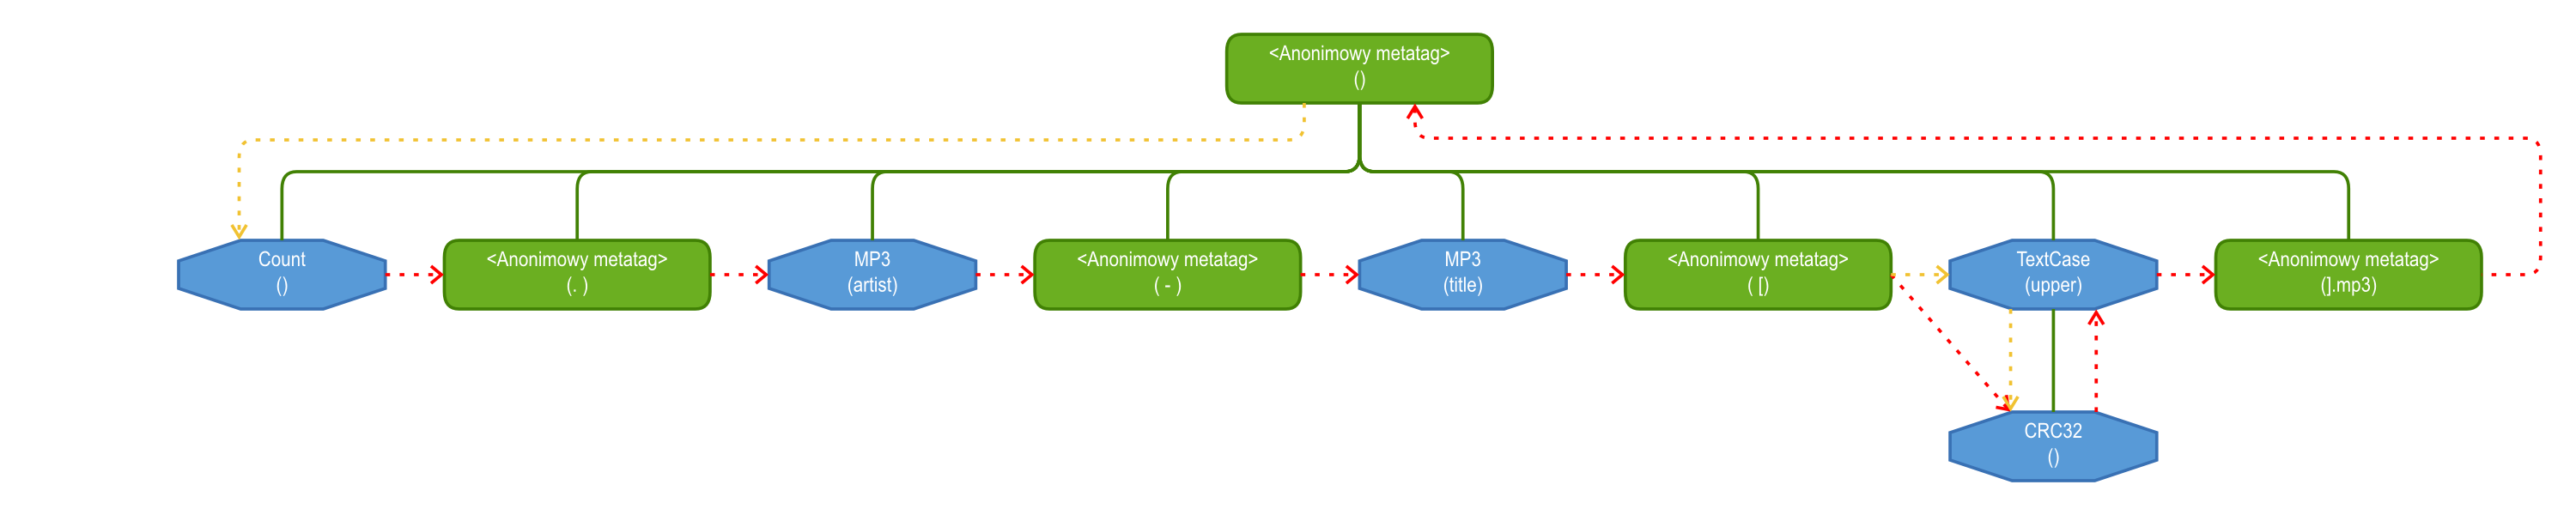
\includegraphics[scale=0.55]{img/metatag_expr_tree4.png}
\end{center}
\caption{Drzewo wywołań stworzone z~przykładowego metawyrażenia}
\label{metatag-expr-tree}
\end{sidewaysfigure}

\par
Drzewo wywołań składa się jedynie z~metatagów. Aby otrzymać taką strukturę, ciągi surowego tekstu (nie będące metatagami) zostają zamienione na wywołania anonimowych (nienazwanych) metatagów, których argumentami inicjalizującymi są właśnie surowe ciągi tekstu, a~jedyną funkcją --- zwrócenie argumentów z~listy inicjalizującej. Dzięki temu ewaluacja wyrażeń jest prostsza, a~dodatkowy anonimowy metatag może zostać wykorzystany na przykład do zmiany kodowania.
\par
Rysunek \ref{metatag-expr-tree} ukazuje strukturę drzewa zbudowanego z~przykładowego wyrażenia z~rysunku \ref{metatag-expr}. Widoczna tu jest wygenerowana hierarchia, na której szczycie znajduje się anonimowy tag. Pojedynczy korzeń ułatwia parsowanie i~wpasowuje się w~logiczną strukturę wyrażenia które nawet nie zagnieżdżone może składać się z~kilku następujących po sobie elementów.
\par
Przy ewaluacji drzewo wywołań przeszukiwane jest w~głąb (co zostało zaznaczone żółtą przerywaną linią), a~jego elementy są ewaluowane od lewej do prawej przy czym metawyrażenia zagnieżdżone w~zakresach operacyjnych (zawierających się między klamrami '\{' i '\}') innych wyrażeń są ewaluowane przed otaczającym je metatagiem-rodzicem. Kolejność ewaluacji jest widoczna na rysunku \ref{metatag-expr-tree} i~oznaczona czerwoną, przerywaną linią. W~ten sposób rezultat wykonania pod-wyrażenia jest dostępny dla tagu-rodzica, co pozwala na wiązanie wywołań niespotykane w~żadnym istniejącym programie tego typu.
\par
Każdy obiekt metatagu musi być zgodny z~interfejsem klasy \texttt{MetatagBase}, która zawiera następujące metody wymagające implementacji:
\begin{enumerate}
\item \texttt{void initialize(const UnicodeString \&arguments)}
\item \texttt{UnicodeString execute(const UnicodeString \&area\_of\_effect)}
\end{enumerate}

Pierwsza z~metod zostaje wywołana na obiekcie podczas łączenia drzewa wywołań z~listą fabryk metatagów i~pobiera jako parametr łańcuch znaków będący zawartością nawiasów tuż po nazwie metatagu. Proces tego typu nazywany jest często \textit{bindowaniem} (od ang. \textit{bind}).\\
Metoda \texttt{execute} wywoływana jest za każdym razem podczas ewaluacji wyrażenia dla danego pliku. Jej argumentem jest zakres operacyjny (opcjonalne pod-wyrażenie zawarte w~nawiasach klamrowych za listą argumentów).\\
Obie metody mogą wyrzucać wyjątki informując o~niepoprawnym argumencie lub błędzie ekstrakcji metadanych.

\section{System modułów}
\label{system-modulow}
\par
Aby ułatwić proces projektowania a~także zwiększyć rozszerzalność aplikacji, duża część funkcjonalności została oddelegowana do oddzielnych modułów zwanych również wtyczkami.
Wtyczki są klasami ładowanymi w~trakcie działania programu z~bibliotek dynamicznych.
W~celu udostępnienia aplikacji funkcjonalności zawartych w~modułach wtyczek, niezbędne było zaprojektowanie menadżera wtyczek --- szablonu \texttt{DynamicPluginManager}.
Klasy menadżera wtyczek umożliwiają programiście-użytkownikowi ładowanie modułów z~wcześniej zadeklarowanym interfejsem niezależnie od platformy systemowej na której uruchamiany jest program\footnote{Same moduły muszą być skompilowane pod platformę na której program ma być uruchamiany.}.

\par
Problemem który rozwiązuje menadżer wtyczek jest fakt że biblioteki dynamiczne  sprawdzają się najlepiej do przechowywania kodu; klasy które istnieją jedynie na etapie kompilacji nie mogą zostać wyeksportowane do pliku jak ma to miejsce w~językach wspierających introspekcje/refleksje typów --- takich jak Java czy C\#.
Aby umożliwić ładowanie wtyczek w~języku C++ należy najpierw zdefiniować czym właściwie jest sama wtyczka.\\

W~MRU (jak i~wielu innych programach) wtyczka jest obiektem udostępniającym metody określone przez interfejs wtyczki. Także biblioteka dynamiczna musi w~jakiś sposób udostępnić owe obiekty.

\par
Menadżer wtyczek po załadowaniu biblioteki dynamicznej przeszukuje ją w poszukiwaniu (zdefiniowanej na poziomie interfejsu wtyczki) funkcji służącej do rejestracji wtyczek. Gdy takową znajdzie, jest ona wywoływana (w kontekście biblioteki dynamicznej) w celu rejestracji fabryk które będą tworzyć instancje wyeksportowanych wtyczek.
Fabryki są potrzebne z dwóch powodów: pierwszym z nich jest fakt że nie zawsze istnieje potrzeba tworzenia wtyczki --- aplikacja może ładować wiele fabryk wtyczek metatagów ale nie wszystkie z nich będą wykorzystywane w wyrażeniu.
Zmniejsza to obciążenie pamięciowe programu jak i~ułatwia pracę twórcom wtyczek, którzy mogą skupić się na implementowaniu faktycznej funkcjonalności modułów. Takie rozwiązanie pozwala również programowi-hostowi na decydowanie w~jakiej ilości i~kiedy mają być tworzone wybrane obiekty.
Drugim powodem jest problem występujący przy alokacji pamięci między modułami --- aplikacja (host) i moduł biblioteki dynamicznej mogą posiadać osobne sterty, przez co nie istnieje możliwość stworzenia wtyczki w bibliotece, a zwolnieje jej w aplikacji hoście. Dlatego też fabryki w MRU są odpowiedzialne również za de-alokacje pamięci.

\section{Typy modułów w~MRU}
\label{moduly}
Aplikacja obsługuje cztery interfejsy wtyczek:
\begin{itemize}
\item UiPlugin --- moduły interfejsu --- pozwalają na implementacje różnych interfejsów użytkownika.
\item InputPlugin --- moduły wejścia --- dostarczają programowi ścieżek do wybranych plików.
\item OutputPlugin --- sterowniki wyjścia --- odpowiadają za faktyczną zmianę identyfikatorów i tworzenie struktury katalogów w systemie plików.
\item MetatagPlugin --- moduły metatagów używanych w wyrażeniach.
\end{itemize}

\section{Moduły UI}
\par
Wtyczki interfejsu użytkownika pozwalają użytkownikowi końcowemu na interakcję z~programem.
Pojedynczy proces aplikacji może posiadać aktywny tylko jeden moduł UI. 
%Decyzja o~wyborze interfejsu użytkownika dokonywana jest na podstawie pliku konfiguracyjnego lub odpowiedniego przełącznika linii poleceń.
Wtyczki interfejsu odpowiadają za całkowitą komunikację między użytkownikiem i~rdzeniem aplikacji (MruCore). One także udostępniają większość funkcjonalności narzędzia, a~także informują użytkownika o~jego stanie i postępie działań.
\par
Jako że funkcjonalność aplikacji jest w~dużej mierze determinowana przez klasę rdzenia (MruCore), interfejs \texttt{UiPlugin} nie posiada z~góry zdefiniowanych metod jak inne wtyczki. Jedyna metoda w~nim zawarta --- \texttt{start} --- pozwala na reinterpretacje linii poleceń i~służy do przekazania kontroli nad programem właśnie do samej wtyczki.

\subsection{wxWidgetsUi}
\par
\texttt{wxWidgetsUi} jest implementacją graficznego interfejsu użytkownika opartego na wspomnianej bibliotece \texttt{wxWidgets}. Założeniem tego modułu jest udostępnienie użytkownikowi końcowemu prostego oraz szybkiego dostępu do funkcjonalności programu, a~także pomoc w~zapoznaniu się z~aplikacją.

\begin{figure}
\begin{center}
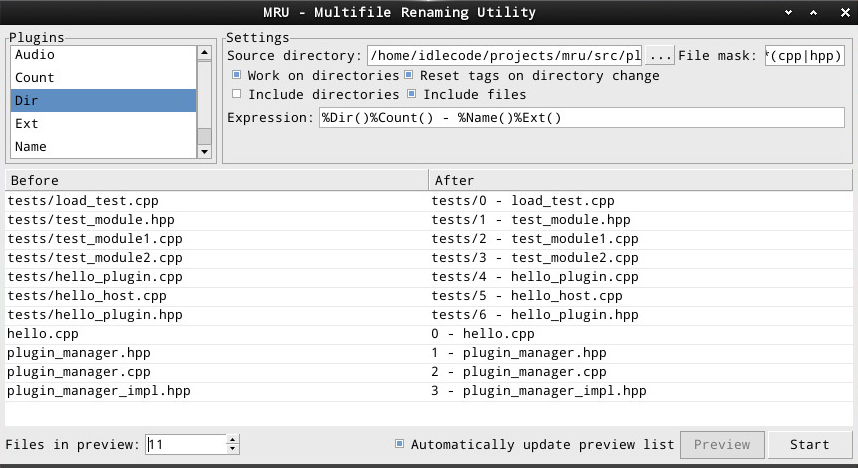
\includegraphics[scale=0.50]{img/wxwidgetsui.png}
\end{center}
\caption{Okno aplikacji MRU --- wtyczka wxWidgetsUi}
\end{figure}

%TODO update:
Okno aplikacji stworzone przez wtyczkę \texttt{wxWidgetsUi} jest podzielone na trzy sekcje:
\begin{itemize}
\item Sekcja górna odpowiada za selekcję plików oraz pozwala na edycję metawyrażenia które ma zostać zastosowane na wybranych plikach.
W~lewym górnym rogu widnieje lista dostępnych Metatagów, a~pola po prawej stronie pozwalają na wybór katalogu, filtru glob oraz samego metawyrażenia.

\item Środkowa część okna stanowi podgląd wybranych plików jak i~efektów zastosowania edytowanego wyrażenia do nich. Lista plików może być ograniczona i~odświeżana w~zależności od opcji znajdujących się pod nią.

\item Na dole okna widoczne są przyciski do (ręcznego) generowania podglądu, jego konfiguracji, a~także rozpoczęcia transformacji nazw dla wybranych plików.
\end{itemize}

%\subsection{TextUi}
%\par
%TextUi jest wtyczką interfejsu udostępniającą funkcjonalność programu z~poziomu linii komend. Pozwala ona na przekazanie parametrów konfiguracyjnych i~rozpoczęcie transformacji nazw bez interakcji z~użytkownikiem jak ma to miejsce w~przypadku graficznych interfejsów użytkownika. Dzięki zastosowaniu tej wtyczki istnieje możliwość wykorzystania aplikacji MRU z~poziomu skryptów powłoki, na maszynach nie wykorzystujących środowiska graficznego lub zdalnych.

\section{InputPlugin}
\par
Jako że biblioteka standardowa języka C++ nie udostępnia mechanizmów pozwalających na iteracje po katalogach, aplikacja musi korzystać z dodatkowych bibliotek lub API systemu operacyjnego. W celu izolacji kodu zależnego od platformy i zmniejszenia zależności rdzenia aplikacji, MRU korzysta z wtyczek wejścia --- \texttt{InputPlugin} --- odpowiedzialnych za iteracje po wybranym przez użytkownika katalogu.
\par
Interfejs wtyczki wejścia pozwala aplikacji na jej prostą konfiguracje (wybór typów plików do iteracji i poziomu przeszukiwania), a także udostępnia iterator --- \texttt{FileIterator} --- generujący kolejne ścieżki do wybranych plików.
\subsection{Dekoratory iteratora}
\par
W przypadku użycia 'surowego' iteratora plików\footnote{Problem występował przynajmniej przy użyciu wtyczki \texttt{BoostInput} opartej na module \texttt{boost::filesystem}} problemem okazała się kolejność generowanych ścieżek oraz typy plików przez nie wskazywanych.
O ile iterator faktycznie generował poprawne ścieżki, to ich kolejność nie odpowiadała choćby leksykalnej kolejności plików w katalogu. Istnieje wiele sytuacji w których pozycja pliku nie wpływa na generowanie identyfikatora, jednak metatagi takie jak \ref{CountTag} biorą ją pod uwagę. Oczywistym rozwiązaniem zdaje się być sortowanie wejściowej listy ścieżek lecz w przypadku dużych kolekcji może to stanowić zbyt duży narzut czasowo-pamięciowy i jak wcześniej zostało wspomniane --- nie zawsze zachodzi potrzeba sortowania. Aby umożliwić użytkownikowi sortowanie wejściowej listy plików zastosowano dekorator \texttt{SortingFileIterator}, który można podłączyć lub odłączyć w zależności od wyboru użytkownika.
%TODO dodać info o predykacie komparatora?

\par
Kolejnym problemem było zwracanie przez iterator praktycznie wszystkich plików znajdujących się w wybranym katalogu. Użytkownik aplikacji powinien mieć możliwość określenia które pliki mają podlegać zmianie.\\
Dzięki wykorzystaniu dekoratora filtrującego \texttt{FilteringFileIterator} aplikacja może wykorzystać dowolny predykat do dynamicznego sprawdzenia czy plik powinien znaleźć się na liście wejściowej.
%TODO dodać info o kolejności łączenia dekoratorów?

\section{Moduł OutputPlugin --- BoostOutput}
\par
Aby wygenerowane identyfikatory mogły zastąpić już istniejące w w systemie plików, powstał interfejs wtyczki \texttt{OutputPlugin}. Jego zadaniem jest udostępnienie aplikacji podstawowych operacji na plikach: kopiowania, przenoszenia, tworzenia i usuwania katalogów.
Istotne jest że wtyczka wyjścia wcale nie musi ingerować w strukturę drzewa plików --- stosując wtyczkę zapisującą informacje do pliku tekstowego, możliwe jest wygenerowanie raportu zawierającego metadane wybranych plików.


\section{Moduły metatagów}
\par
Główna funkcjonalność aplikacji została zawarta w~modułach tagów --- to one odpowiadają za ekstrakcje metadanych lub generowanie wartości, które rdzeń aplikacji jedynie składa i~przesyła wraz z~komunikatem zmiany do modułu wyjścia.
\par
Każdy z~poniżej wymienionych tagów może zostać dodany do wyrażenia po załadowaniu odpowiedniej biblioteki dynamicznej go zawierającej
%\footnote{Część tagów nie wymaga ładowania --- są wbudowane w~plik wykonywalny aplikacji, natomiast część mimo iż jest dostarczana w~standardzie z~aplikacją może wymagać dodatkowej konfiguracji w~postaci określenia ścieżki ładowania bibliotek}.

\subsection{Count}
\par
Metatag \texttt{Count} jest używany do numeracji wybranych plików.
Dla każdego pliku generowany jest kolejny numer. Lista argumentów tagu pozwala na określenie wartości początkowej oraz kroku iteracji.
W~poniższej tabeli zawarte zostały parametry obsługiwane przez metatag:
\begin{table}[h]
\begin{center}
\begin{tabular}{| c | p{13cm} |}
\hline
\textbf{Argument} & \textbf{Opis} \\
\hline
start=\textit{N} & Ustawia początkowy stan licznika na \textit{N}--- od tej wartości tag rozpocznie zliczanie \\
step=\textit{K} & Ustawia rozmiar kroku --- kolejny numer będzie większy o~\textit{K} w~stosunku do poprzedniego \\
\hline
\end{tabular} \end{center}
\caption{Zestaw argumentów inicjalizacyjnych dla metatagu \texttt{Count}}
\end{table}

Aby wykorzystać kilka argumentów jednocześnie należy oddzielić je od siebie za pomocą symbolu przecinka --- '\texttt{,}'.

\subsection{Audio}
\par
Metatag \texttt{Audio} został oparty na bibliotece \texttt{TagLib} i~pozwala na ekstrakcję metadanych z~wielu plików multimedialnych.
Tag ten obsługuje następujące argumenty:
\begin{table}[h]
\begin{center}
\begin{tabular}{| c | p{13cm} |}
\hline
\textbf{Argument} & \textbf{Opis} \\
\hline
title & Ekstrakcja tytułu utworu \\
artist & Ekstrakcja nazwy artysty wykonującego utwór \\
album & Ekstrakcja nazwy albumu w~którym zawiera się utwór \\
year & Ekstrakcja roku powstania utworu \\
comment & Ekstrakcja komentarza \\
\hline

\end{tabular}
\caption{Zestaw argumentów inicjalizacyjnych dla metatagu \textsf{Audio}}
\end{center}
\end{table}

\subsection{Name}
\par
Metatag \texttt{Name} reprezentuje źródłową nazwę pliku bez rozszerzenia oraz katalogu zawierającego. Może być używany gdy zachodzi potrzeba dodania prefiksu lub sufiksu do istniejącej nazwy pliku. Dzięki składni metawyrażeń możliwa jest również modyfikacja źródłowego identyfikatora na przykład za pomocą tagu TextCase.

\subsection{Ext}
\par
Metatag \texttt{Ext} reprezentuje rozszerzenie pliku. Jako że modyfikacja rozszerzenia może prowadzić to błędnej interpretacji pliku przez inne programy, często jest niepożądana. Metatag \texttt{Ext} użyty na końcu metawyrażenia stosowany jest w~celu zachowania rozszerzenia pliku.

\subsection{Dir}
\par
\texttt{Dir} jest metatagiem reprezentującym ścieżkę w~której znajduje się przetwarzany plik. Ścieżka zwracana przez \texttt{Dir} jest ścieżką pośrednią w~stosunku do katalogu przetwarzania wybranego przez użytkownika --- dla plików znajdujących się bezpośrednio w~wybranym katalogu, metatag \texttt{Dir} zwraca pusty tekst.

\subsection{TextCase}
\par
Metatag \texttt{TextCase} jest używany do zmiany wielkości liter w~skojarzonym z~tagiem zakresie działania. Pewność działania dla pełnego zakresu kodów unicode jest zapewniona dzięki wykorzystaniu funkcji z~biblioteki ICU.

%\subsection{Convert}


\begin{table}[h]
\begin{center}
\begin{tabular}{| c | p{13cm} |}
\hline
\textbf{Argument} & \textbf{Opis} \\
\hline
upper & Wszystkie znaki w~zakresie zostaną zamienione na ich większe odpowiedniki \\
lower & Wszystkie znaki w~zakresie zostaną zamienione na ich mniejsze odpowiedniki \\
title & Wszystkie znaki w~zakresie zostaną zamienione tak by wyglądały na tytuł (Pierwsze znaki każdego słowa są zamieniane na ich większe odpowiedniki \\
\hline
\end{tabular} \end{center}
\caption{Zestaw argumentów inicjalizacyjnych dla metatagu \texttt{TextCase}}
\end{table}

\section{Testy}
\label{testy}

\par
 W~celu przetestowania aplikacji ze strony \url{http://www.jamendo.com/pl/track/986557/pulsar} zostało pobrane archiwum zawierające album muzyczny z~plikami w~formacie \textit{MPEG-1/MPEG-2 Audio Layer 3} --- popularnie zwanym '\textit{MP3}' --- które to zawierają poprawnie sformatowane tagi ID3 w~wersji 2.4.0.\\
Celem testu było sprawdzenia parsera metawyrażeń, filtra regex, a~także ogólnego działania programu.
Na rysunku \ref{test-before} widać stan katalogu przed uruchomieniem programu.

\begin{figure}[h]
\begin{center}
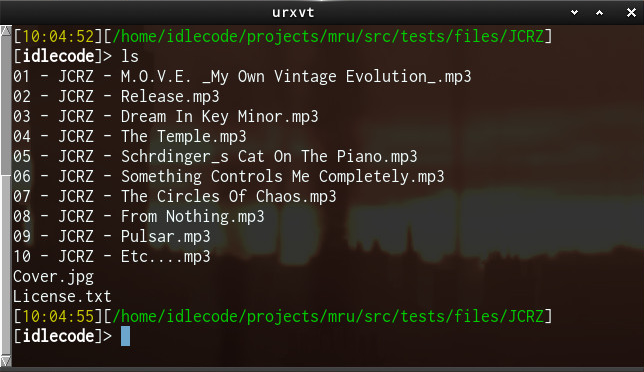
\includegraphics[scale=0.70]{img/test_before.png}
\end{center}
\caption{Stan plików przed zmianą}
\label{test-before}
\end{figure}

\par
Do testów zostało wybrane metawyrażenie wykorzystujące metatagi Audio, TextCase oraz Ext.
Celem użytego metawyrażenia jest kompozycja nazwy składającej się z~nazwy albumu do którego utwór należy (metatag \texttt{\%Audio(album)}) pisanej dużymi literami, po której następuje tytuł (\texttt{\%Audio(title)}) oraz rok wydania utworu w~nawiasach kwadratowych (\texttt{[\%Audio(year)]}). Wykorzystany na końcu metatag Ext, zapewnia że pliki wynikowe będą posiadały takie samo rozszerzenia jak w~nazwa źródłowa.\\
Dodatkowo w~celu zmniejszenia ilości błędów został zastosowany filtr z~wyrażeniem regularnym "\textit{.*mp3}", który zapewnia że program będzie przetwarzać jedynie pliki zakończone ciągiem znaków "\textit{mp3}".

\begin{center}
\texttt{\%TextCase(upper)\{\%Audio(album)\} - \%Audio(title) [\%Audio(year)]\%Ext()}
\end{center}

\begin{figure}[h]
\begin{center}
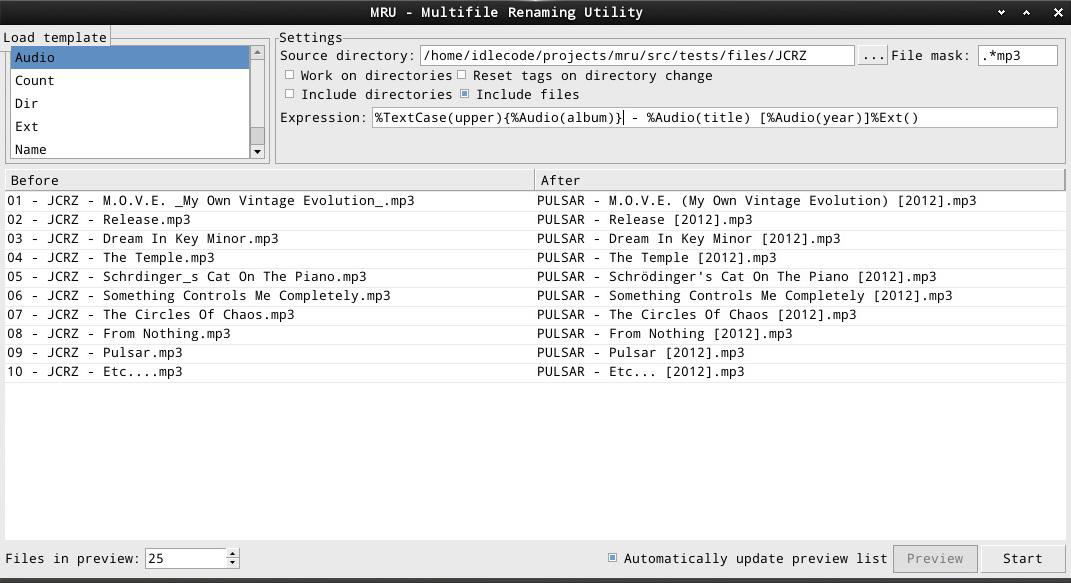
\includegraphics[scale=0.45]{img/test_window.png}
\end{center}
\caption{Konfiguracja aplikacji użyta do zmiany identyfikatorów}
\end{figure}

\begin{figure}[h]
\begin{center}
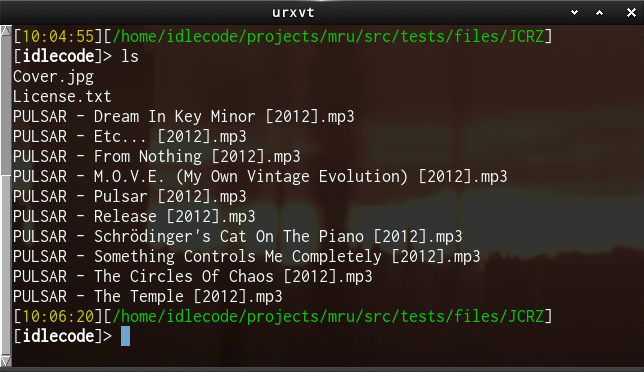
\includegraphics[scale=0.70]{img/test_after.png}
\end{center}
\caption{Stan plików po zmianie}
\end{figure}

\section{Możliwości rozwoju i~ponownego wykorzystania komponentów}
\par
Dzięki zastosowanej architekturze modułowej, części aplikacji nie posiadają dużych zależności między-modułowych co stwarza idealne warunki do ich rozwoju i~ponownego użycia istniejącego kodu (na przykład wtyczek) w~innych projektach.

\par
System wtyczek został zaimplementowany w~formie biblioteki niezależnej od platformy i~nie posiadającej rozwiązań specyficznych dla aplikacji w~której został wykorzystany. Dzięki temu jego wykorzystanie w~innych projektach nie wymaga dodatkowego narzutu związanego z~modyfikacją kodu.

\par
Moduły metatagów wymagają jedynie dostępu do pliku na którym mają operować i~same nie są świadome metawyrażeń w~których występują. Dzięki zastosowanie takiej izolacji, dodawanie nowych wtyczek nie wywiera wpływu na działający program, a~istniejące metatagi mogą zostać wykorzystane z~powodzeniem w~innych aplikacjach, które wymagają dostępu do metadanych. Dzięki spójnemu interfejsowi, metatagi mogą stanowić alternatywę dla wykorzystywania dedykowanych bibliotek do obsługi formatów plików, które często zawierają sporo narzutu związanego z~funkcjami bezpośrednio nie związanymi z~danymi --- jak na przykład zapisem faktycznych danych.\\
Metatagi (szczególnie generujące sumy kontrolne) mogą znaleźć również zastosowanie przy porównywaniu plików w~celu identyfikacji duplikatów.

\par
Wtyczki wyjścia --- OutputPlugin --- nie mają w~żaden sposób narzuconej implementacji.
%Ich zadaniem jest jedynie udostępnienie iteratora do faktycznych plików.
Nic więc nie stoi na przeszkodzie aby stworzyć wtyczkę która generuje na przykład tekstowe raporty dla istniejących plików zawierające metadane w~nich zawarte.
